\section{segmentation}
This chapter will go through how the segmentation of the sound was achieved, the segmentation is needed to find where there is a sound so that all of the input are not interpitated as one sound.\\
In the transcription system the segmentation was made by calculated the RMS and making a threshold saying that once the RMS value can over a certain value it would not be considered as noise but as a sound. \\
\begin{figure}[h]
	\begin{center}
		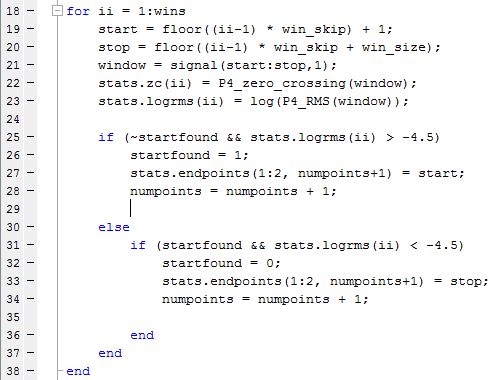
\includegraphics[scale =  0.8]{fig/Find_Endpoint_script.png}
		\caption{part of the code that will find the endpoint}
		\label{P4_Findendpoints}
	\end{center}
\end{figure}
The code for finding endpoint are shown on figure \ref{P4_Findendpoints} in the for loop the full signal are analysed in a window size and window skip that are given in the functions input. Inside each window the signal are analysed for what the RMS is over that window. With the value the next operation that will take place inside the for loop is two if statements, the first if statement will check if the threshold have not been passed and if the RMS value are above the threshold if so we tell the system that a signal have started, next the place in samples where the signal has started will be placed in a vector. The other if statement will act when there has been detected a signal and when the signal go below the threshold then this place is noted in the vector that also has the start, also the value that say we have found a signal will be change to 0 as the program can see that the signal has ended.\\
For feature analysis the part of the signal marked are put into a vector plus the onset time and the duration of the sounds.\\
So to sum up the segmentation in our transcription system are made by making a threshold on the RMS values.